%
% bloecke.tex
%
% (c) 2021 Prof Dr Andreas Müller, OST Ostschweizer Fachhochschule
%
\bgroup
\def\sx{1}
\def\sy{0.1}
\def\block#1#2{
	\fill[color=red] ({#1},{-#1}) rectangle ({#1+#2},{-#1-#2});
}
\def\kreuz#1{
	\draw[color=white,line width=0.1pt] (0,{-#1})--(60,{-#1});
	\draw[color=white,line width=0.1pt] (#1,0)--(#1,-60);
}
\definecolor{darkgreen}{rgb}{0,0.6,0}
\begin{frame}[t]
\frametitle{Blockgrössen aus $\dim\mathcal{K}^k(A)$ ablesen}
\vspace{-20pt}
\begin{columns}[t,onlytextwidth]
\begin{column}{0.56\textwidth}
\begin{center}
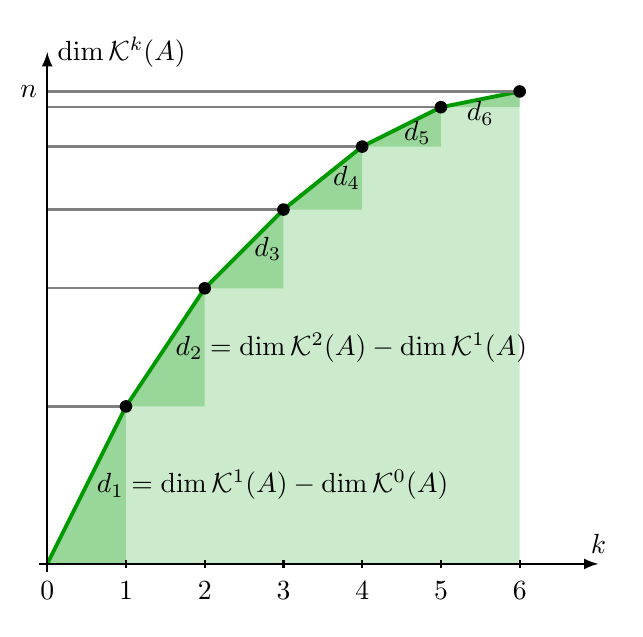
\begin{tikzpicture}[>=latex,thick]

\coordinate (A) at ({1*\sx},{20*\sy});
\coordinate (B) at ({2*\sx},{(20+15)*\sy});
\coordinate (C) at ({3*\sx},{(20+15+10)*\sy});
\coordinate (D) at ({4*\sx},{(20+15+10+8)*\sy});
\coordinate (E) at ({5*\sx},{(20+15+10+8+5)*\sy});
\coordinate (F) at ({6*\sx},{(20+15+10+8+5+2)*\sy});
\fill[color=darkgreen!20] (0,0) -- (A) -- (B) -- (C) -- (D) -- (E) -- (F)
	-- ({6*\sx},0) -- cycle;

\fill[color=darkgreen!40] (0,0) -- ({1*\sx},0) -- (A) -- cycle;
\fill[color=darkgreen!40] (A) -- ({2*\sx},{20*\sy}) -- (B) -- cycle;
\fill[color=darkgreen!40] (B) -- ({3*\sx},{(20+15)*\sy}) -- (C) -- cycle;
\fill[color=darkgreen!40] (C) -- ({4*\sx},{(20+15+10)*\sy}) -- (D) -- cycle;
\fill[color=darkgreen!40] (D) -- ({5*\sx},{(20+15+10+8)*\sy}) -- (E) -- cycle;
\fill[color=darkgreen!40] (E) -- ({6*\sx},{(20+15+10+8+5)*\sy}) -- (F) -- cycle;

\draw[color=darkgreen,line width=1.4pt] (0,0) -- (A) -- (B) -- (C) -- (D) -- (E) -- (F);

\draw[color=gray] (A) -- (0,{20*\sy});
\draw[color=gray] (B) -- (0,{(20+15)*\sy});
\draw[color=gray] (C) -- (0,{(20+15+10)*\sy});
\draw[color=gray] (D) -- (0,{(20+15+10+8)*\sy});
\draw[color=gray] (E) -- (0,{(20+15+10+8+5)*\sy});
\draw[color=gray] (F) -- (0,{(20+15+10+8+5+2)*\sy});

\node at ({0.5*\sx},{0.5*20*\sy})
	[right] {$d_1 = \dim\mathcal{K}^1(A)-\dim\mathcal{K}^0(A)$};
\node at ({1.5*\sx},{0.5*(20+20+15)*\sy})
	[right] {$d_2 = \dim\mathcal{K}^2(A)-\dim\mathcal{K}^1(A)$};
\node at ({2.5*\sx},{0.5*(2*20+2*15+1*10)*\sy}) [right] {$d_3$};
\node at ({3.5*\sx},{0.5*(2*20+2*15+2*10+8)*\sy}) [right] {$d_4$};
\node at ({4.5*\sx-0.1},{0.5*(2*20+2*15+2*10+2*8+5)*\sy+0.2}) [below right] {$d_5$};
\node at ({5.5*\sx},{0.5*(2*20+2*15+2*10+2*8+2*5+2)*\sy+0.1}) [below] {$d_6$};

\fill (A) circle[radius=0.08];
\fill (B) circle[radius=0.08];
\fill (C) circle[radius=0.08];
\fill (D) circle[radius=0.08];
\fill (E) circle[radius=0.08];
\fill (F) circle[radius=0.08];

\draw[->] (-0.1,0) -- ({6*\sx+1},0) coordinate[label={$k$}];
\draw[->] (0,-0.1) -- (0,6.5) coordinate[label={right:$\dim\mathcal{K}^k(A)$}];

\foreach \x in {0,1,...,6}{
	\draw ({\sx*\x},{-0.05}) -- ({\sx*\x},0.05);
	\node at ({\sx*\x},{-0.1}) [below] {$\x$};
}

\node at (0,{60*\sy}) [left] {\llap{$n$}};

\end{tikzpicture}
\end{center}
\end{column}
\begin{column}{0.43\textwidth}
\vspace{-10pt}
\begin{center}
\begin{tabular}{>{$}c<{$}|>{$}r<{$}|>{$}c<{$}|>{$}c<{$}}
k&d_k&\# M_k(\Bbbk)\text{-Blöcke}&\text{Beispiel}\\
\hline
0&  0&        &\\
1& 20& d_1-d_2&5\\
2& 15& d_2-d_3&5\\
3& 10& d_3-d_4&2\\
4&  8& d_4-d_5&3\\
5&  5& d_5-d_6&3\\
6&  2& d_6    &2\\
\end{tabular}
\end{center}
\vspace{-13pt}
\begin{center}
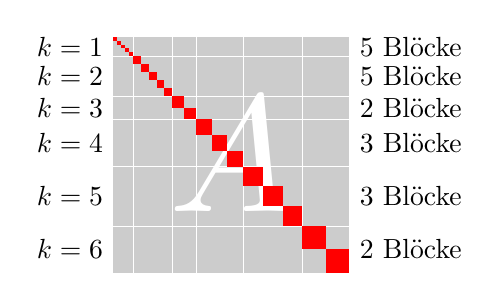
\begin{tikzpicture}[>=latex,thick,scale=0.05]
\fill[color=gray!40] (0,0) rectangle (60,-60);
\node[color=white] at (30,-30) [scale=6] {$A$};
\kreuz{5}
\kreuz{15}
\kreuz{21}
\kreuz{33}
\kreuz{48}
\node at (0,-2.5) [left] {$k=1$};
\node at (60,-2.5) [right] {$5$ Blöcke};
\node at (0,-10) [left] {$k=2$};
\node at (60,-10) [right] {$5$ Blöcke};
\node at (0,-18) [left] {$k=3$};
\node at (60,-18) [right] {$2$ Blöcke};
\node at (0,-27) [left] {$k=4$};
\node at (60,-27) [right] {$3$ Blöcke};
\node at (0,-40.5) [left] {$k=5$};
\node at (60,-40.5) [right] {$3$ Blöcke};
\node at (0,-54) [left] {$k=6$};
\node at (60,-54) [right] {$2$ Blöcke};
\block{0}{1}
\block{1}{1}
\block{2}{1}
\block{3}{1}
\block{4}{1}
\block{5}{2}
\block{7}{2}
\block{9}{2}
\block{11}{2}
\block{13}{2}
\block{15}{3}
\block{18}{3}
\block{21}{4}
\block{25}{4}
\block{29}{4}
\block{33}{5}
\block{38}{5}
\block{43}{5}
\block{48}{6}
\block{54}{6}
\end{tikzpicture}
\end{center}
\end{column}
\end{columns}
\end{frame}
\egroup
